\subsection{Central Limit Theorem}


Under certain conditions, the normal distribution can be used to approximate probabilities for linear combinations of random variables having a non-normal distribution. This follows from the Central Limit Theorem (C.L.T.). 

The normal distribution is commonly used because it tends to approximate the distribution of sums of random variables.


\begin{theorem}[\textbf{Central Limit Theorem}]
    \phantom{}  \\
    If $X_1, X_2, \ldots, X_n$ are \textbf{independent} random variables all having the \textbf{same distribution},
    with mean $\mu$ and variance $\sigma^2$, then as $n \to \infty$, the cumulative distribution
    function (c.d.f.) of the random variable
    \[{\color{blue} Z \approx} \frac{\dis \sum_{i=1}^n X_i - n\mu}{\sigma \sqrt{n}} = \frac{S_n - n\mu}{\sigma \sqrt{n}}\]
    approaches the $N(0, 1)$ cumulative distribution function. Similarly, the cumulative distribution
    function of 
    \[{\color{blue} Z \approx} \frac{\overline{X} - \mu}{\frac{\sigma}{\sqrt{n}}}\]
    approaches the $N(0, 1)$ cumulative distribution function.
\end{theorem}

\begin{remark}
    For large $n$, we have
    \begin{itemize}
        \item $S_n = \displaystyle \sum_{i=1}^{n} X_i \sim \text{N}(n\mu, n\sigma^2)$.
        \item $\overline{X} = \frac{1}{n} \displaystyle \sum_{i=1}^{n} X_i \sim \text{N}(\mu, \frac{\sigma^2}{n})$.
    \end{itemize}
    If $X_i$'s themselves have normal distributions, then $S_n$ and $\overline{X}$ have \textbf{exactly} normal distributions $\forall n$. Otherwise, $S_n$ and $\overline{X}$ have \textbf{approximately} normal distributions.
\end{remark}

\pagebreak

\begin{note}
    \phantom{}
    \begin{itemize}
        \item Although this theorem is about limits, we will use it when $n$ is large, but finite.
        \item This theorem works for all distributions except those whose $\mu$ and $\sigma^2$ do not exist.
        \item The accuracy of the approximation depends on $n$ (bigger is better) and on the actual distribution $X_i$'s. It works for small $n$ when $X_i$'s p.d.f. is close to symmetric.
    \end{itemize}
\end{note}

\begin{theorem}[\textbf{The Law of Large Numbers}]
    \phantom{}\\
    Draw simple random samples of size $n$ at random from a large population with mean $\mu$. As the number of observations drawn increases (i.e. as $n \to \infty$), then the sample mean $\overline{X}$ approaches the population mean $\mu$.
\end{theorem}

General idea of the C.L.T. is that it takes any distribution and makes it normal.
\begin{figure}[htbp]
    \center
    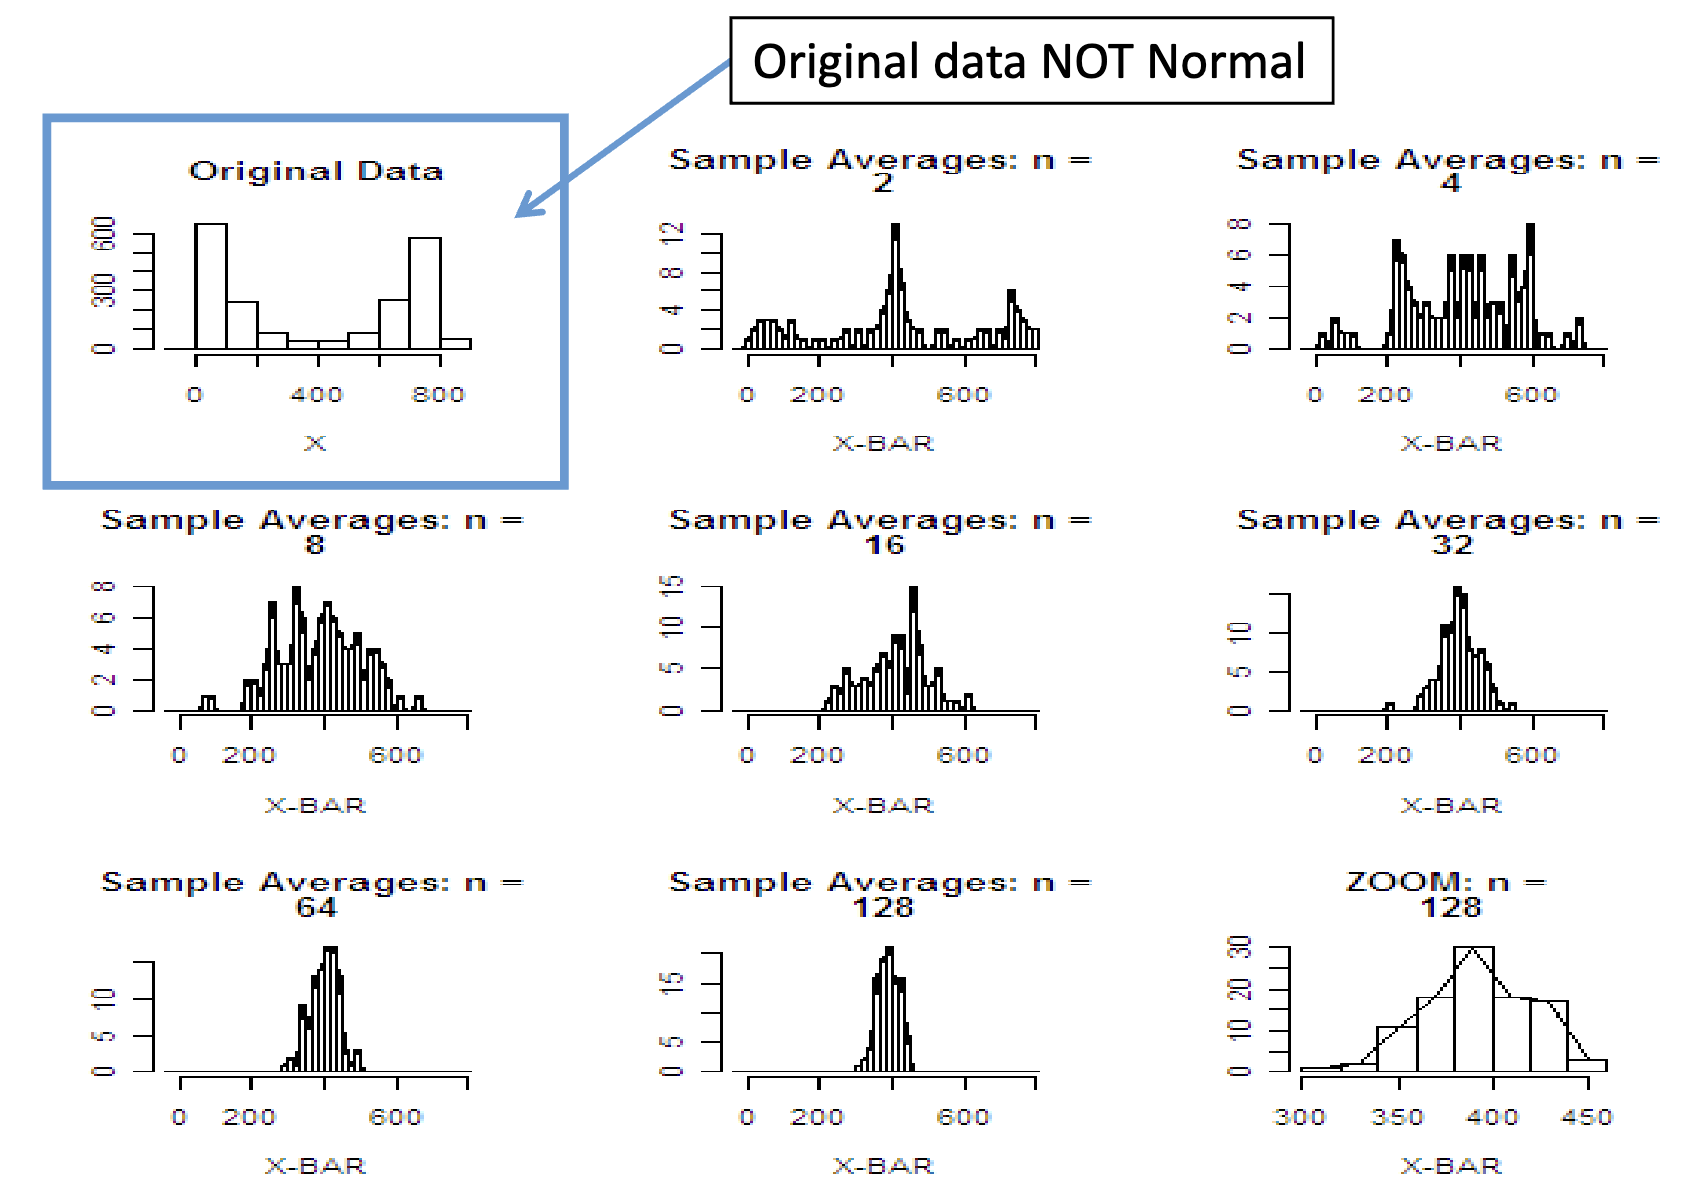
\includegraphics[scale=0.4]{img/CLT-ex.png}
    \caption{Visualizing the idea of CLT.}
\end{figure}

\begin{note}
    The distribution of sample means becomes normal as the sample size increases. Also, the sample mean converges to the population mean when $n$ becomes larger.
\end{note}


\pagebreak


\begin{example}
    Suppose fires reported to a fire station satisfy the conditions for a Poisson process, with a mean of 1 fire every 4 hours. Find the probability the $500^{\text{th}}$ fire of the year is reported on the $84^{\text{th}}$ day of the year.

    \textbf{Solution:} Let $X_i =$ time beteen $(i-1)^{\text{st}}$ and the $i^{\text{th}}$ fires ($X_1 =$ time to the first fire). Then, these $X_i$'s are independent and identically distributed as: $X_i \sim \text{Exp}(\theta = 4 \text{ hrs} = \frac{1}{6} \text{ day})$, since $\lambda = \frac{1}{4}$ fires per hour.

    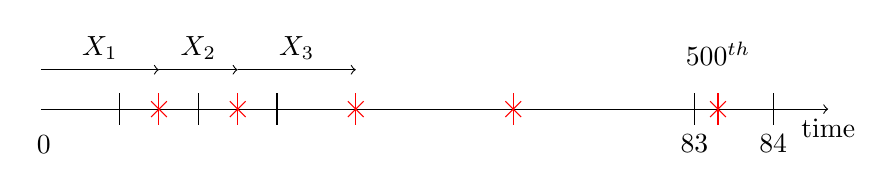
\begin{tikzpicture}
        % Draw the horizontal axis
        \draw[->] (0,0) -- (10,0) node[anchor=north] {time};
        
        % Draw the vertical lines and labels
        \foreach \x in {1, 2, 3} {
            \draw (\x,0.2) -- (\x,-0.2);
        }
        
        % Draw the crosses and labels for 83 and 84
        \foreach \x in {1.5, 2.5, 4, 6, 8.6} {
            \draw[red] (\x,0.2) -- (\x,-0.2);
            \draw[red] (\x-0.1,0.1) -- (\x+0.1,-0.1);
            \draw[red] (\x-0.1,-0.1) -- (\x+0.1,0.1);
        }
        
        \draw (8.3,0.2) -- (8.3,-0.2) node[anchor=north] {83};
        \draw (9.3,0.2) -- (9.3,-0.2) node[anchor=north] {84};
        
        % Draw the arrows for X1, X2, X3
        \draw[->] (0,0.5) -- (1.5,0.5) node[midway,above] {$X_1$};
        \draw[->] (1.5,0.5) -- (2.5,0.5) node[midway,above] {$X_2$};
        \draw[->] (2.5,0.5) -- (4,0.5) node[midway,above] {$X_3$};
        \node at (8.6,0.7) {$500^{\text{th}}$};
        
        % Add the 0 and 1 labels on the left
        \node[anchor=east] at (0.25,-0.45) {0};
        % \node[anchor=east] at (0.78,-0.45) {1};
    \end{tikzpicture}

    We want to find $P \left( 83 < \underbrace{\displaystyle \sum_{i=1}^{500} X_i}_{S_{500}} \leq 84 \right)$. By the Central Limit Theorem, $S_{500} = \displaystyle \sum_{i=1}^{500} X_i$ has approximately \vspace{-2mm}

    a $\text{N}(500\mu , 500\sigma^2) = \text{N}(\frac{500}{6}, \frac{500}{36})$ distribution. 
    \begin{align*}
        P(83 < S_{500} \leq 84) &\approx P \left( \frac{83 - \frac{500}{6}}{\sqrt{\frac{500}{36}}} < Z \leq \frac{84 - \frac{500}{6}}{\sqrt{\frac{500}{36}}} \right) \\
        &= P(-0.09 < Z \leq 0.19) \\
        &\vdots \\
        &= 0.57142 + 0.53586 - 1 \\
        &= 0.10728.
    \end{align*}
\end{example}

\begin{note}
    In this example, we used the normal distribution to approximate a continuous random variable (i.e. the exponential distribution). When approximating discrete random variables, we have to make a small adjustment, see next page!
\end{note}


\pagebreak


\begin{remark}[\textbf{Continuity Correction}]
    \phantom{}\\
    When approximating a discrete random variable, a slight adjustment is required to improve the approximation. 

For example, we are in a `100-cup challenge', we bought 100 cups to see how many times we win. We want to find the probability of having between 15 to 20 winning cups. 

Let $X_i = $ whether the $i^{\text{th}}$ cup is a winning cup. Then $X_i \sim \text{Binomial}(n=1,p=\frac{1}{6})$ for $i = 1,2,\ldots,100$. And $\expect{X_i} = \frac{1}{6}$, $\Var{X_i} = \frac{5}{36}$, with $S_{100} = \displaystyle \sum_{i=1}^{100} X_i = $ total number of winning cups. By the CLT, we have $S_{100}$ approximately have $\text{N}(\frac{100}{6}, \frac{500}{36})$, we'll see a theorem below about this. Then,
\[
    P(15 \leq S_{100} \leq 20) = P(-0.447 \leq Z \leq 0.894) = 0.487.
\]
If we compute the exact probability using $S_{100} \sim \text{Binomial}(100, \frac{1}{6})$, we get $P(15 \leq S_{100} \leq 20) = 0.561$. This is quite off!

Since $X_i$ are discrete, so $S_{100}$ is also discrete and cannot take non-integer values. In this case, the approximation is underestimate as seen in Figure 14 (part of $X=15$ and $X = 20$ are not included by the normal approximation in {\color{blue} blue}), so subtract 0.5 to get $P(14.5 \leq S_{100} \leq 20.5)$, which gives a better approximation.

\begin{figure}[!htb]
    \begin{minipage}{0.5\textwidth}
      \centering
      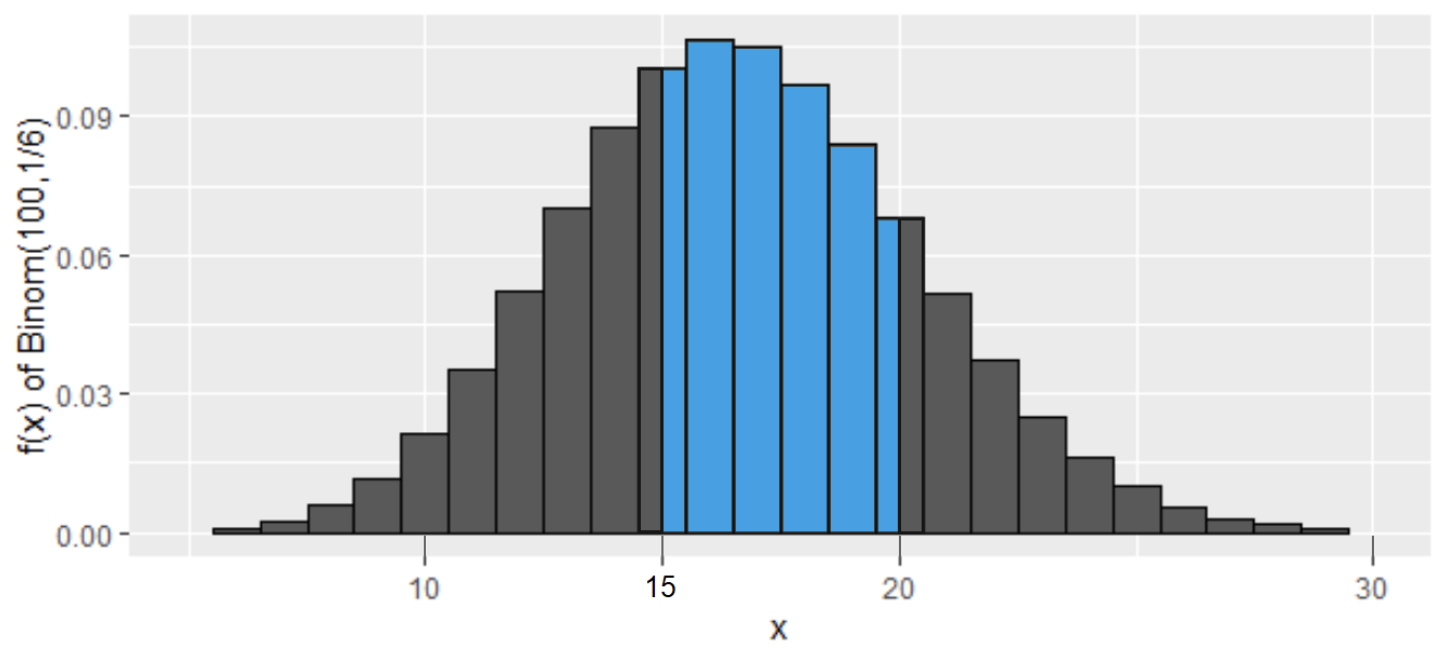
\includegraphics[width=1\linewidth]{img/without-adjustment.png}
      \caption{Without adjustment (underestimate).}
    \end{minipage}\hfill
    \begin{minipage}{0.5\textwidth}
      \centering
      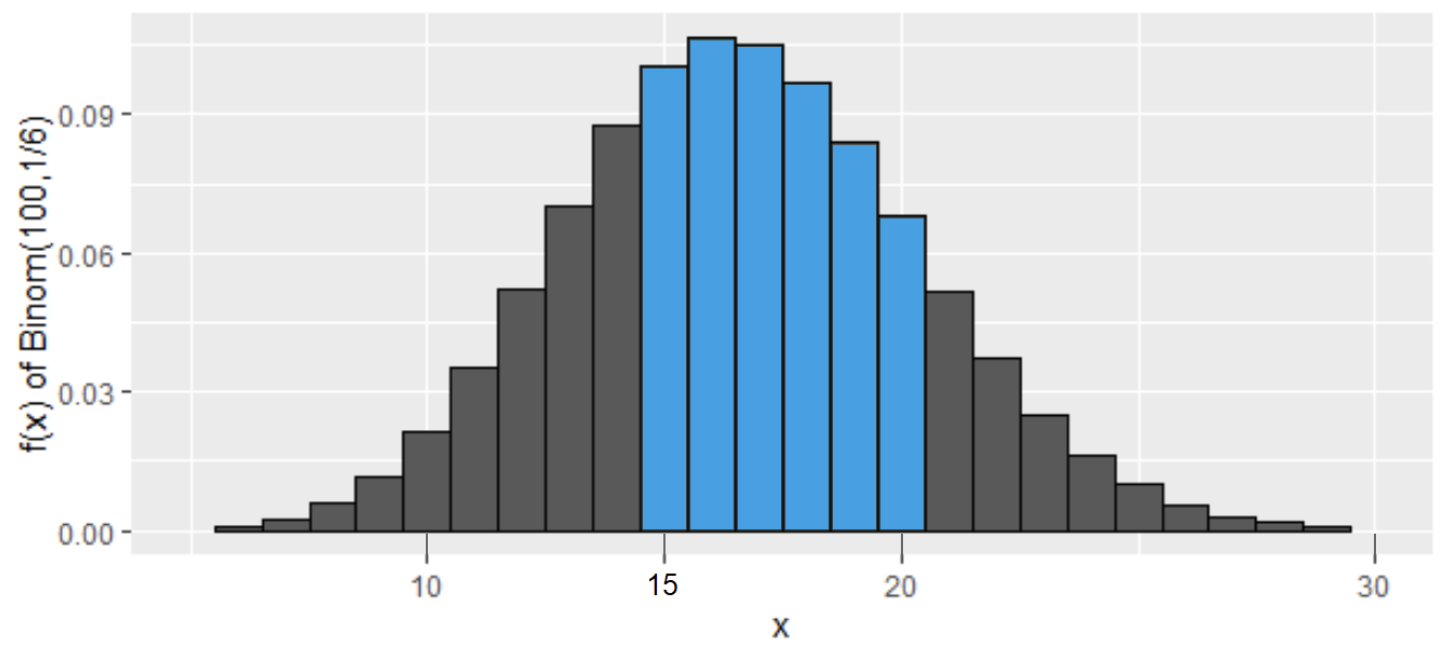
\includegraphics[width=1\linewidth]{img/with-adjustment.png}
      \caption{With adjustment (better).}
    \end{minipage}
 \end{figure}

 $P(14.5 \leq S_{100} \leq 20.5) = 0.568$, which is way better!

 This adjustment is called the ``\textbf{Continuity Correction}''.
\end{remark}

\begin{note}
    \phantom{}
    \begin{itemize}
        \item It is only applied when using a \textbf{continous} distribution to approximate a \textbf{discrete} one.
        \item Quick sketch to see whether to add or subtracct 0.5 (see below proposition).
    \end{itemize}
\end{note}

\begin{proposition}[\textbf{Continuity Correction Rules}]
    \phantom{}\
    \begin{itemize}
        \item $P(X > n)$, use $P(X > n + 0.5)$.
        \item $P(X \geq n)$, use $P(X > n - 0.5)$.
        \item $P(X > n)$, use $P(X < n - 0.5)$.
        \item $P(X \leq n)$, use $P(X < n + 0.5)$.
        \item $P(a < X < b)$, use $P(a + 0.5 \leq X \leq b - 0.5)$.
        \item $P(a \leq X \leq b)$, use $P(a - 0.5 \leq X \leq b + 0.5)$.
        \item $P(X = n)$, use $P(n-0.5 \leq X \leq n + 0.5)$.
    \end{itemize}
\end{proposition}

\begin{theorem}[\textbf{Normal Approximation to Poisson}]
    \phantom{}  \\
    Suppose $X \sim Poisson(\mu)$. Then the cumulative distribution function of the standarized
    random variable \vspace{-2mm}
    \[Z = \frac{X - \mu}{\sqrt{\mu}}\]
    approaches that of a standard Normal random variable as $\mu \to \infty$.
\end{theorem}

\begin{remark}
    We have $X \sim \text{N}(\mu,\mu)$, where $\mu = \lambda t$. Approximation will be good when $\mu > 5$.
\end{remark}

\begin{theorem}[\textbf{Normal Approximation to Binomial}]
    \phantom{}  \\
    Suppose $X \sim Binomial(n, p)$. Then for large $n$, the random variable \vspace{-1mm}
    \[W = \frac{X - np}{\sqrt{np(1 - p)}}\]
    has approximately a $N(0, 1)$ distribution.
\end{theorem}

\begin{remark}
    We write $\frac{X - np}{\sqrt{np(1 - p)}} \sim \text{N}(0,1)$ or $X \sim \text{N}(np,np(1-p))$. \vspace{-1mm} \\
\end{remark}


\begin{example}
    Suppose $X \sim \text{Poi(9)}$. Use the Normal approximation to approximate $P(X > 9)$, and cpmare with the true value.

    By above theorem, we have $Z = \frac{X-\mu}{\sqrt{\mu}}$. Using continuity correction, \vspace{-3mm}
    \[
        P(X > 9) \approx P(X > 9 \text{ } {\color{blue} + \text{ } 0.5}) = P \left( Z > \frac{9.5 - 9}{\sqrt{9}} \right) = P(Z > 0.17) = 0.4324.
    \]
    Note: the true value is 0.4126.
\end{example}

\subsection{Moment Generating Functions}

So far, we have seen two functions which characterize a distribution of a random variable:
\begin{itemize}
    \item p.d.f.
    \item c.d.f.
\end{itemize}
However, there is a third function which also \textbf{uniquely} determines a distribution: the \textbf{moment generating function}.


\begin{definition}[\textbf{Moment Generating Functions}]
    \phantom{}\\
    Consider a discrete random variable $X$ with probability function $f(x)$. The moment generating function (m.g.f.) of $X$ is defined as \vspace{-3mm}
    \[
        M(t) = \expect{e^{tX}} = \displaystyle \sum_{\text{all $x$}} e^{tx} f(x).
    \]
    We will assume that the moment generating function is defined and finite for values of $t$ in an interval around 0 (i.e. for some $a > 0$, $\displaystyle \sum_{x} e^{tx} f(x) < \infty \; \forall t \in [-a,a]$).
\end{definition}

The m.g.f. of $X$ can be used to evaluate the moments of the random variable $X$, where the \textbf{moments} of $X$ are defined as the \textbf{expectations} of the functions $X^k$ for $k = 1,2,\ldots$. \vspace{-3mm}
\[
    \expect{X^k} \text{ is the $k^{\text{th}}$ moment of $X$.}
\]

\begin{example}
    \phantom{}\
    \begin{itemize}
        \item The mean $\mu = \expect{X}$ is the first moment of $X$.
        \item $\expect{X^2}$ is the second moment of $X$ and so on.
    \end{itemize}
\end{example}


\begin{theorem}
    \phantom{}\\
    Suppose the random variable $X$ has moment generating function $M(t)$ defined $\forall t \in [-a,a]$ for some $a > 0$. Then \vspace{-3mm}
    \[
        \expect{X^k} = 
    \]
\end{theorem}



\subsection{Motivariate Moment Generating Functions}









\newpage